%!TEX root=Principal.tex
\chapter{CLASSIFICADOR BAYESIANO DO USUÁRIO}
\label{cap:proposta}

Nos capítulos anteriores é possível identificar que a existência de robôs em ambientes sociais torna-se cada vez mais comum no dia-a-dia das pessoas. Como qualquer produto existente no mercado, é necessário que os robôs proporcionem uma boa experiência aos usuários durante o uso, que nesse caso é o convívio em ambiente doméstico ou industrial. Entretanto, as técnicas difundidas em interação humano computador, que tem o objetivo de aumentar a experiência positiva do usuário em produtos tecnológicos, são pouco aplicadas por pesquisadores na área de robótica social, de serviço e assistiva~\cite{alenljung:2017}.

Dado o cenário onde a melhora da interação pode ser alcançada através do uso das técnicas de interação humano computador, com as de usabilidade, essa tese apresenta um classificador bayesiano do perfil de usuário baseado em técnicas de Personas e heurísticas de avaliação de interface unidas ao sentimento de conforto, desconforto e medo do usuário ao interagir com o robô. O intuito é fazer com que o robô a partir da classificação do usuário possa identificar como se relacionar com aquele perfil no futuro. A partir desse ponto é esperado que o robô possa deixar o usuário a vontade enquanto convivem no mesmo ambiente. O trabalho apresentado nessa seção, serve como guia para a evolução do classificador de usuário. O uso desse classificador unificado a uma técnica de adaptação de comportamento e aprendizado é capaz de ajudar na experiência de usuário positiva. As técnicas utilizadas são: (I) Personas, técnica utilizada para representar um grupo de usuários através de um personagem fictício que possui o perfil médio do grupo; (II) Heurísticas de Nielsen utilizadas para avaliação da interface de um sistema, foram adaptadas para a interação humano-robô. Elas auxiliam o robô a medir variáveis sobre a experiência do usuário na interação; e (III) \emph{Proxemics}, teoria de proximidade (vide seção~\ref{cap:proxemics}), que estuda o comportamento de agentes sociais de acordo com a distância entre si.

Outro ponto importante apresentado na literatura, é sobre a cultura da pessoa. A cultura influência diretamente o comportamento de uma pessoa em ambientes sociais. Isso significa que algumas reações apresentadas por pessoas no ambiente social são influenciadas pelo seu local de nascimento, pelos locais onde viveu e, consequentemente, pela sua experiência de vida. Fatores como a experiência de vida e cultura são difíceis de avaliar apenas através da observação. Conseguir fazer com que uma pessoa tenha liberdade para contar esse tipo de informação necessita de interações de longo prazo, podendo levar meses até compreender toda história dessa pessoa. Algumas questões referentes a cultura do usuário são discutidas nos resultados apresentados no capítulo~\ref{cap:resultados}.

Sendo o robô um produto tecnológico, o uso de técnicas que sejam capazes de aumentar a efetividade da interação, não havendo a necessidade de conhecer por completo a história de vida do indivíduo em questão. Essas técnicas tem o objetivo de deixar o sistema mais fácil de usar e acima de tudo aumentar a experiência, a satisfação do usuário ao utilizá-lo. Para que o robô possa realizar essa classificação e raciocínio sobre as informações que existem no ambiente alguns passos são apresentados ao longo deste capítulo.

Com base no robô disponível para os experimentos, as ações que são possíveis para ele executar são estabelecidas. A seção~\ref{sec:robo} apresenta em detalhes o robô utilizado para essa pesquisa. Na sequência dois questionários são apresentados, o primeiro aplicado antes do teste de interação e o segundo após. O primeiro questionário estabelece o perfil do usuário referente a questões de aderência a tecnologia, contato prévio com robôs, a cultura que ele se identifica e a expectativa em relação a robôs em ambientes domésticos e profissionais. O questionário pós-teste possui informações declaradas sobre o conforto, desconforto, medo e avaliação do comportamento do robô, durante a interação.

Com os questionários definidos, 39 pessoas foram selecionadas para participar do teste de interação com o robô, de acordo com o cenário descrito na seção~\ref{sec:cenario}. Os testes foram executados com o comportamento do robô de maneira aleatória, ou seja, com o mínimo de preocupação com a experiência do usuário neste momento. Coletados os perfis e informações dos usuários, é realizado uma preparação e normalização dos dados para que o algoritmo QG-SIM possa realizar o agrupamento dos perfis similares, conforme o processo apresentado por \citeonline{masiero:2013b}. A partir dos grupos gerados pelo algoritmo QG-SIM, é realizado o processo de criação de Personas~\cite{masiero:2013, masiero:2013b}.

Personas são criadas com base nas informações extraídas de cada grupo através dos questionários de pré e pós teste de interação. O próximo passo, é estabelecer as dependências condicionais entre cada variável aleatória incluida através da análise dos dados e observações dos testes de interação. As variáveis são compostas pelas Personas criadas, algumas heurísticas de Nielsen adaptadas para interação com o robô, a proximidade entre robô e usuário, as ações e comportamentos do robô e efeitos de conforto, desconforto e medo da pessoa durante a interação. Essa dependência condicional entre as variáveis faz com que elas sejam organizadas no formato de uma rede bayesiana. O objetivo dessa rede é classificar qual o perfil do usuário dado que houve um conforto, desconforto e/ou medo durante a interação com o robô em um cenário residencial.

As variáveis aleatórias foram definidas de maneira abstrata e podem, no futuro, sugir outras que auxiliem na classificação do usuário de maneira que o resultado da rede bayesiana possa servir como alimentação de um mecanismo de decisão do robô para melhorar a interação com o usuário. Ao final, um conjunto de variáveis são propostos como pontos para futuras investigações e evolução do classificador entregue por essa tese.

O restante deste capítulo apresenta em detalhes os passos da proposta acima descrita. Ao final do capítulo é apresentado a visão completa do \emph{framework}, onde é realizado uma síntese do processo como um todo e das técnicas aplicadas nele.

\section{Ações e Comportamentos do Robô}
\label{sec:comportamento-robo}
O robô escolhido para os experimentos possui uma série de características que auxiliam a interação social e serviço domésticos, uma vez que ele foi construído para atender a competição de robótica RoboCup@Home~\cite{robocup:2015}. Com base nos atuadores de interação existentes (vide seção~\ref{sec:robo}), foram mapeados as variáveis de ações e comportamentos do robô. A tabela~\ref{tab:variaveisvalores} apresenta as variáveis, compostas por seus respectivos valores.

\begin{table}[!ht]
	\caption{Variáveis de Comportamento do Robô}
	\label{tab:variaveisvalores}
	\centering
	\begin{tabular}{c | c}
		\hline
		Variável & Valor \\
		\hline
		Gestos & curto \\
		& longo \\
		\hline
		Fala & educada \\
		& autoritária \\
		\hline
		Expressão Facial & amigável \\
		& não amigável \\
		\hline
		Proximidade & longe - (Entre Pública e Social ) \\
		& perto - (Entre Pessoal e Íntima ) \\
		\hline
		Velocidade & rápida \\
		& devagar \\
		\hline
		Posição & sentado \\
		& em pé \\
		\hline
	\end{tabular}
	\smallcaption{Fonte: O autor.}
\end{table}

Além das variáveis direcionadas aos atuadores do robô, a tabela~\ref{tab:variaveisvalores} apresenta a variável de proximidade entre o robô e o ser humano e a variável posição que determina como o usuário estava durante a interação, sentado ou em pé. São variáveis importantes, pois auxiliam a determinar o comportamento de reação da pessoa para um mesmo tipo de gesto do robô em diferentes situações. Por exemplo, se o robô encontra-se próximo da pessoa, entre as zonas Pessoal e Íntima, um gesto amplo pode gerar um desconforto maior do que o mesmo gesto ocorrendo entre as zonas Pública e Social. Ou como é a reação do usuário quando o robô aproximar o manipulador próximo ao rosto do usuário.  A partir das variáveis definidas e comportamentos implementados no robô é importante agora trabalhar com os questionários pré e pós testes.

\section{Questionários para Coleta de Dados de Interação}
\label{sec:questionarios}
Para apoiar o processo de obtenção dos resultados e construção dos perfis dos usuários, dois questionários foram construídos. O primeiro, aplicado em momento anterior ao teste, tem como objetivo o mapeamento de informações sobre características físicas que possam ser reconhecidas pelo robô, adesão a tecnologia, contatos prévios com robôs e questões culturais onde o usuário declara quais locais ele possui mais afinidade e quais ele já teve o privilégio de visitar. As questões serão agrupadas de acordo com seus objetivos e apresentadas em listas. Todas as questões a seguir fazem para do questionário pré-teste.

Questões focadas na identificação e características físicas do usuário:

\begin{enumerate}
	\item Informe seu nome completo
	\item e-mail para contato
	\item Informe o número do seu celular
	\item Testes poderão ocorrer usando o Robô no Centro Universitário FEI. Você gostaria de realizar o teste com o robô físico? Opções de resposta: Sim, Não
	\item Qual a sua idade? (em anos)
	\item Qual a sua altura? (em metros)
	\item Informa seu gênero: Opções de resposta: Feminino, Masculino, Prefiro não dizer
	\item Na maior parte do tempo, você se considera uma pessoa com feição: Opções de reposta: Sorridente, Normal, Séria/Fechada
	\item Você se considera uma pessoa sociável? Opções de resposta: Sim, Não
	\item Você utiliza óculos de grau? Opções de resposta: Sim, Não (Obs: Pessoas com lente de contato, por favor, repondam não. A intenção é identificar a armação.)
	\item Você possui cabelo comprido? Opções de resposta: Sim, Não
	\item Qual etnia você se considera? Opções de resposta: Amarela, Branca, Indígena, Parda, Preta, Não declarada
\end{enumerate}

Questões voltadas a informações sobre a adesão à tecnologia:

\begin{enumerate}
	\item Qual(is) dispositivo(s) tecnológico(s) você mais utiliza (marque 1 ou mais opções): Opções de resposta: Celular, Computador (de mesa ou notebook), Tablet, Smart TV, Relógio Smart, MP3 Player, Câmera Fotográfica Digital, Leitor de e-Book, outros
	\item Qual(is) dispositivo(s) tecnológico(s) você nunca utilizou (marque 1 ou mais opções): Opções de resposta: Celular, Computador (de mesa ou notebook), Tablet, Smart TV, Relógio Smart, MP3 Player, Câmera Fotográfica Digital, Leitor de e-Book, Já utilizei todas
	\item Você possui conta em banco digital (ex: Original, Neon, etc.) ? Opções de resposta: Sim, Não
	\item Você possui cartão de crédito digital (ex: Nubank, Digio, etc.) ? Opções de resposta: Sim, Não
	\item Qual o principal meio de pagamento de suas contas? Opções de resposta: Celular, Computador, Tablet, Autoatendimento, Caixa Físico
	\item Você utiliza redes sociais? Opções de resposta: Sim, Não
	\item Quais as redes sociais que você mais utiliza (marque 1 ou mais opções): Opções de resposta: Facebook, Instagram, Twitter, Google\+, Snapchat, outras
\end{enumerate}

Questões culturais:

\begin{enumerate}
	\item Qual foi o local de nascimento? (Informe da seguinte maneira: Cidade; Estado; País)
	\item Em qual local, você viveu por mais tempo durante sua infância e adolescência? (Informe da seguinte maneira: Cidade; Estado; País)
	\item Qual o seu atual local de moradia? (Informe da seguinte maneira: Cidade; Estado; País)
	\item Qual o país que você melhor se identifica com a cultura? (Considere também a opção do seu país de nascimento.)
	\item Qual a cidade, na sua opinião, que melhor representa a cultura que você se identifica (resposta não dependente da questão acima)?
	\item Você visitou outros países, além do Brasil? Opções de resposta: Sim, Não
	\item Quais países você já visitou? (Responda separando os países por ponto e vírgula, ex: França; Estados Unidos; Itália; Japão;)
	\item Aproximadamente, quantas cidades na região nordeste do Brasil você visitou?
	\item Aproximadamente, quantas cidades na região norte do Brasil você visitou?
	\item Aproximadamente, quantas cidades na região centro-oeste do Brasil você visitou?
	\item Aproximadamente, quantas cidades na região sudeste do Brasil você visitou?
	\item Aproximadamente, quantas cidades na região sul do Brasil você visitou?
\end{enumerate}

Por fim, questões sobre contato prévio com robôs:

\begin{enumerate}
	\item Em algum momento de sua vida, você teve contato com robôs? Opções de resposta: Sim, Não
	\item Se sim para a questão anterior, quais tipos de robôs você teve contato (marque 1 ou mais opções): Opções de resposta: Parecido com animais, Parecido com pessoas, Robôs de linha de produção/fábrica, Robôs Móveis (que contém rodas), outros
	\item O que você espera do comportamento do Robô ao tê-lo em sua casa?
	\item O que você espera do comportamento do Robô ao tê-lo em seu trabalho?
	\item Dadas as questões anteriores, gostaria de fazer mais algum comentário sobre você?
\end{enumerate}

O segundo questionário mantém o foco na interação do usuário durante o teste e quais pontos do robô mais agradaram ou não na opinião dele. Além disso, um detalhe do teste que pode impactar na interação também é registrado, se o usuário estava em posição sentada ou em pé. As questões apresentas a seguir compõe o questionário pós-teste:

\begin{enumerate}
	\item Informe o número de amostra (Identificador dos documentos referentes ao comitê de ética)
	\item Você se sentiu confortável durante a aproximação do robô? Escala de 1 à 10
	\item Você se sentiu com medo em algum momento durante a aproximação do robô? Escala de 1 à 10
	\item Você estava \_\_\_\_\_\_\_\_\_ durante a aproximação do robô. Opções de resposta: Sentado, em Pé
	\item Você voltaria a interagir com esse robô novamente? Opções de resposta: Sim, Não
	\item Justifique a resposta anterior.
	\item O que você mais gostou no robô?
	\item O que você menos gostou no robô?
	\item Depois dessa experiência, você interagiria com outros robôs? Opções de resposta: Sim, Não
	\item Você estaria confortável com um robô convivendo em sua casa? Opções de resposta: Sim, Não
	\item Justifique a resposta anterior.
	\item Em algum momento da interação, você se sentiu desconfortável com o comportamento do robô? Opções de resposta: Sim, Não
	\item Descreva o desconforto em caso de sim, na resposta anterior.
	\item Você alteraria algum comportamento apresentado pelo robô durante o teste? Qual?
	\item Observações e comentários:
\end{enumerate}

Os questionários apresentados também auxiliam o processo para definir as probabilidades nas tabelas condicionais das variáveis aleatórias que compõem a rede bayesiana. Todo o processo e questionários apresentados nesse capítulo são aprovados pelo comitê ética sobre identificador de processo CAAE: 70057117.0.0000.5508.

\section{Preparando os dados para o algoritmo QG-SIM}
\label{sec:preparacao}
Com os processos de captura das informações concluídos, é necessário trabalhar na normalização dos dados para que seja possível executar o algoritmo que agrupará os perfis semelhantes. Nesse momento, é necessário uma análise manual para separar as informações. O primeiro passo é deixá-las todas em uma única base de dados, pois encontram-se em duas bases diferentes, pré e pós-teste.

Com as informações reunidas em uma única base de dados, é necessário remover informações de texto livre uma vez que o algoritmo não possui um interpretador semântico e fica difícil criar um modelo quantitativo para essas informações, de maneira que exista um sentido de comparação entre as respostas.

As informações quantitativas existentes, como por exemplo a idade do usuário, pode-se aplicar a distância euclidiana ou alguma outra distância de acordo com a necessidade do projeto. No caso do agrupamento de perfis desta tese, a distância euclidiana é adotada já que atende por completo a necessidade do algoritmo e do processo.

Em relação as variáveis categóricas, ou seja, as variáveis que possuem um valor textual separadas por categoria, existem duas opções para converte-las em valores quantitativos. A primeira opção é inserir um código númerico para cada valor, por exemplo, os valores ``Celular, Computador, Tablet, Autoatendimento, Caixa Físico'' recebem um valor representado por um número inteiro cada ficando ``Celular = 1, Computador = 2, Tablet = 3, Autoatendimento = 4, Caixa Físico = 5'', conforme~\citeonline{masiero:2013}. A segunda opção é transformar essas variáveis em \emph{dummies}~\footnote{http://pandas.pydata.org/}. O método \emph{dummies} transforma cada opção de resposta em uma variável binária onde o valor 1 é para quando a opção foi selecionada e 0 para o oposto.

Nesse ponto a base de dados está com todas as variáveis quantificadas, porém existe um segundo problema que pode afetar o resultado do algoritmo. Cada variável possui uma escala diferente. Essa diferença na escala das variáveis pode gerar tendências no resultado do algoritmo, assim é necessário padronizar os valores númericos existentes na base. Para realizar a padronização dos dados o processo de normalização é executado. A normalização mais comum a ser feita é manter os valores das variáveis entre 0 e 1~\cite{lattin:2011}. A equação~\ref{eq:normalizacao1} apresenta a forma mais simples de realizar o processo de normalização dos dados. É feita a divisão do valor da característica pelo valor máximo encontrado entre a característica analisada.

\begin{equation}
	X_{i_{normalizado}} = \frac{X_i}{\max_{X_i}}
	\label{eq:normalizacao1}
\end{equation}

Entretanto, o uso da equação \ref{eq:normalizacao1} para normalizar os dados, pode gerar também uma tendência ou generalização da normalização. Pode existir uma concentração dos dados em um determinado intervalo generalizando a informação coletada~\cite{masiero:2013}. Para evitar o problema da concentração dos dados, utiliza-se a equação \ref{eq:normalizacao2} como método mais efetivo na normalização dos dados.

\begin{equation}
	X_{i_{normalizado}} = \frac{X_i - \min_{X_i}}{\max_{X_i} - \min_{X_i}}
	\label{eq:normalizacao2}
\end{equation}

Após o processo de normalização, as escalas da base estão com uma distribuição uniforme e prontas para serem consumidas pelo algoritmo.

\section{Executando o QG-SIM e criando as Personas}
\label{sec:criarpersonas}
Com as informações normalizadas, o próximo passo é executar o algoritmo de agrupamento QG-SIM. A implementação do algoritmo pode ser encontrada no endereço \url{https://github.com/amasiero/qgsim}. O algoritmo solicita um valor de similaridade mínimo para manter a qualidade entre os elementos de um mesmo grupo. Esse valor é chamado de Q. A partir desse valor, o QG-SIM irá agrupar os perfis de acordo com a similaridade desejada e irá gerar o número de grupos automaticamente~\cite{masiero:2013}.

Assim que os grupos são definidos, é necessário encontrar a medida de dispersão central para cada uma das variáveis do perfil. As medidas de dispersão mais comuns são: média, mediana e moda. Elas auxiliarão no processo de construção da Persona, como definição da idade, se utiliza óculos, tipo do cabelo, gênero, e outras informações. Como os grupos encontrados não possuiam ruídos em sua distribuição, a medida de disperção adota foi a média (vide capítulo~\ref{cap:resultados}). Nesse momento, as informações de texto livres preenchidas são utilizadas como base para preencher a descrição e história da Persona. É verificado cada resposta dos indivíduos que compõe o grupo e na sequência é criado todo uma história de vida para a Persona.

Nesse processo, cinco Personas foram encontradas e são apresentadas a seguir:
\begin{table}[!ht]
	\caption{Persona Joaquim}
	\label{tab:joaquim}
	\centering
	\begin{tabular}{ m{2 cm} | m{13cm} }
		\hline
		Foto: & \rule{0cm}{2.7cm} 
\includegraphics[scale=0.8]{joaquim.png} \\
		\hline
		Nome: & Joaquim \\
		\hline
		Descrição: & Tem 21 anos, 1,71 m de altura, em geral não é uma pessoa séria ou carrancuda, mas também não é sorridente. É um homem sociável, cheio de amigos a sua volta e adora ir ao barzinho com eles. Mora na capital paulista, centro econômico brasileiro, local perfeito para um homem que gosta de variedade cultural. Não fica longe de seu smartphone e também sempre que pode, está com seu laptop no colo navegando pelo Facebook e postando fotos no Instagram. Tudo que pode ser resolvido pelo seu smartphone ele faz, seja por chamada de voz ou qualquer aplicativo. Mas, ainda não conseguiu se habituar aos serviços financeiros digitais, prefere o método clássico para guardar seu dinheiro, o colchão. Nunca viajou para fora do Brasil, inclusive seu mapa de viagens nacionais também não é extenso. Ao todo, visitou apenas 9 cidades do Brasil com o passar do tempo.

		Na universidade acompanhou os times de robótica nas competições e teve contato com diversos tipos de robôs, como os parecidos com humanos e animais, com mobilidade através de rodas e também os de linha de produção. Quando perguntam sua expectativa sobre robôs convivendo em sua casa, ele diz que tudo bem, desde que ele execute as tarefas domésticas sempre com obediência e de certa maneira, também espera que o robô seja afetivo na interação. Um comportamento próximo ao de uma diarista na família. Já no ambiente industrial, Joaquim acredita que os robôs são apenas ferramentas de trabalho e não devem fazer nada além de executar o que lhe foi programado. \\
		\hline
	\end{tabular}
	\smallcaption{Fonte: O autor.}
\end{table}

\begin{table}[!ht]
	\caption{Persona Maria Eduarda}
	\label{tab:mariaeduarda}
	\centering
	\begin{tabular}{ m{2 cm} | m{13cm} }
		\hline
		Foto: & \rule{0cm}{2.7cm} 
\includegraphics[scale=0.8]{maria_eduarda.png} \\
		\hline
		Nome: & Maria Eduarda \\
		\hline
		Descrição: & Aos 36 anos, com 1,71 m de altura, é uma garota reservada que adora sorrir em diversas ocasiões. É bem sociável, e mantém os amigos por perto. É uma mulher moderna e gosta de manter seu corte de cabelo mais curto que o convencional. Mora em São Bernardo do Campo, cidade da grande São Paulo e gosta muito de visitar o interior de São Paulo para passar seus feriados prolongados. Não vive sem seu celular, e no trabalho o computador é sua principal ferramenta. Quando está em casa utiliza sua Smart TV para assistir suas séries e filmes favoritos. Gostario muito de ter um leitor de e-book para evitar carregar livros pesados durante seu trajeto pelo transporte público. Mesmo com essa adoção a tecnologia, empresas digitais, principalmente do mercado financeiro, não a atraem. Sempre conectada através do celular, ela posta tudo no Facebook, tanto de trabalho quanto de lazer.

		Já viajou algumas vezes para os EUA, sempre a passeio com o principal destino a Disney. Pelo Brasil, já viajou para algumas cidades fora de São Paulo e deixou sua marca por todas as regiões do país. Como ela trabalha em uma universidade de engenharia, já viu diversos tipos de robôs, que são utilizados nas aulas. Porém, nunca teve um contato direto com eles, a não ser seu aspirador de pó. Tanto em casa quanto no trabalho, ela espera que robôs sejam capazes de realizar tarefas com eficácia, como dirigir um carro, digitar planilhas, mas que ao mesmo tempo não seja capaz de substituí-la.\\
		\hline
	\end{tabular}
	\smallcaption{Fonte: O autor.}
\end{table}

\begin{table}[!ht]
	\caption{Persona Alfredo}
	\label{tab:alfredo}
	\centering
	\begin{tabular}{ m{2 cm} | m{13cm} }
		\hline
		Foto: & \rule{0cm}{2.7cm} 
\includegraphics[scale=0.8]{alfredo.png} \\
		\hline
		Nome: & Alfredo \\
		\hline
		Descrição: & Aos 24 anos, rapaz de estatura normal, por volta de 1,75m, está sempre com um belo sorriso no rosto, faça chuva ou faça sol. Sempre tem pessoas a sua volta, gosta de contar piadas e fazer todos sorrirem. Morador da cidade de São Bernardo do Campo, mas sempre que pode vai para o litoral paulista visitar os pais e curtir uma praia. Usa computador para fazer os trabalhos da faculdade e passa grande parte do seu tempo no celular. Não possui serviços financeiros digitas, pois ainda não conseguiu a aprovação do cadastro. Quando se trata de internet banking, acredita que o seu computador é mais seguro que o uso de celular.

		Alfredo vive antenado nas redes sociais, como Twitter, Instagram e Facebook. Ajudam ele a ficar conectado com as últimas notícias e eventos a sua volta. Tem um sonho de viajar para o exterior, mas isso ainda não foi possível, em compensação pelo Brasil já visitou mais de 30 cidades, a maioria na região Sudeste. Na universidade, através do curso de engenharia de automação, teve contato com robôs de fábrica e móveis conforme os laboratórios das disciplinas ocorriam. Qunado perguntam a Alfredo o que ele espera de um robô doméstico e também um robô no trabalho, ele diz que robôs devem executar as tarefas propostas de maneira eficiente e que seu interação seja toda por comando de voz.\\
		\hline
	\end{tabular}
	\smallcaption{Fonte: O autor.}
\end{table}

\begin{table}[!ht]
	\caption{Persona Danielo}
	\label{tab:danielo}
	\centering
	\begin{tabular}{ m{2 cm} | m{13cm} }
		\hline
		Foto: & \rule{0cm}{2.7cm} 
\includegraphics[scale=0.8]{danielo.png} \\
		\hline
		Nome: & Danielo \\
		\hline
		Descrição: & Com 27 anos de idade, 1,83m, Danielo está sempre na academia para treinar com seus amigos. Mora em São Bernardo do Campo, e utiliza seu computador para fazer seu trabalho e o celular para manter contato com seus amigos. Nunca quis saber de leitores de e-book, pois acha sua tecnologia sem utilidade nos dias atuais. A sua única rede social é o Facebook. Ele acha que já toma tempo o suficiente e não precisa de outras para ver a mesma coisa. Danielo é um rapaz que já viajou bastante. Já visitou 3 países latinos e no Brasil visitou mais de 90 cidades, concetradas em sua grande parte, na região Sudeste. O contato com robôs é limitado e restrito a robôs de fábrica. Em casa ele acredita que o robô será parecido com seres humanos para fazer as atividades domésticas, e no trabalho substituirão seres humanos em trabalhos repetitivos, como nas fábricas e linha de produção.\\
		\hline
	\end{tabular}
	\smallcaption{Fonte: O autor.}
\end{table}

\begin{table}[!ht]
	\caption{Persona Manuel}
	\label{tab:manuel}
	\centering
	\begin{tabular}{ m{2 cm} | m{13cm} }
		\hline
		Foto: & \rule{0cm}{2.7cm} 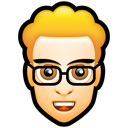
\includegraphics[scale=0.8]{manuel.png} \\
		\hline
		Nome: & Manuel \\
		\hline
		Descrição: & Aos 33 anos, 1,85 m,  Manuel um professor universitário sempre sorridente. Seus alunos sempre o procuram para esclarecer dúvidas e pedir conselhos. Mora em São Bernardo do Campo, próximo ao seu local de trabalho, por que adora o conforto de ir em sua casa poder almoçar uma comida fresca. Acredita que tem uma melhor qualidade de vida assim. Não é muito fã de tecnologia de ponta, então fica contente em ter seu computador, onde resolve tudo que pode. Digitalmente, considera-se antisocial e não mantém cadastro em nenhuma rede social.

		Já visitou paises pela Europa, África, América do Norte e do Sul. No Brasil, seu foco de visitar está na região Sudeste, principalmente o estado de Minas Gerais. No total já percorreu mais de 62 cidades pelo país. Como professor, sua linha linha de pesquisa principal de estudos é a robótica, fazendo com que tenha contato com todos os tipos de robôs. Em casa, pensa em ter um robô para atender suas necessidades, assim como no trabalho. Porém, o robô no trabalho deve atender também as necessidades e expectativas da empresa.\\
		\hline
	\end{tabular}
	\smallcaption{Fonte: O autor.}
\end{table}

As Personas apresentadas nas tabelas~\ref{tab:joaquim}, \ref{tab:mariaeduarda}, \ref{tab:alfredo}, \ref{tab:danielo}, \ref{tab:manuel} foram criadas com base nas informações coletadas no formulário e auxiliaram na definição das independências condicionais da rede bayesiana. Mais informações das avaliações feitas com base nas Personas sobre a interação com o robô são apresentadas no capítulo~\ref{cap:resultados}.

\section{Heurísticas adaptadas de Nielsen}
\label{sec:heuristicas}
Avaliação heurística é um método utilizado principalmente por especialistas em usabilidade para verificar problemas de interação em interfaces de sistemas. Ao longo dos tempos, as 10 heurísticas de Nielsen são as mais utilizadas nesse tipo de avaliação (vide seção~\ref{sec:avaliacao}). Dessa forma, é apresentado uma adaptação das heurísticas de Nielsen focado em sistemas robóticos sociais. É importante essa adaptação, pois elas serão analisadas e a proposta é que o próprio robô saiba que a utilizou e faça uma  autoavaliação do seu comportamento para a experiência de usuário durante a interação. Assim, ele pode identificar se o usuário teve algum desconforto ou medo e assim melhorar seu comportamento através de outras técnicas de inteligência artificial e aprendizado de máquina. As adaptações das heurísticas são:

\begin{itemize}
	\item \textbf{Visibilidade do status do robô}: o robô deve sempre manter o humano informado sobre o que está acontecendo por meio de feedback apropriado dentro de um tempo razoável. O status do sistema deve ser exposto constantemente para o humano durante movimentação ou parado. O feedback pode ser gerado via voz ou algum outro método visual. Não fornecer feedback sobre o status do sistema quando o robô encontra-se estático, causa desconforto ao humano. \textbf{Uso na tese}: No robô utilizado para os testes os usuários questionaram sobre o alerta de alguns comportamentos, além do uso das expressões faciais, voz e gestos como ferramenta de status. Essa é uma heurística que influencia diretamente na avaliação do comportamento do robô na interação então deve fazer parte da rede bayesiana.
	\item \textbf{Equivalência entre o robô e o mundo real}: o robô deve usar a linguagem do usuário com palavra, frases e conceitos que lhe sejam familiares, ao invés de termos orientados à tecnologia. Deve-se seguir convenções do mundo real, fazendo a informação aparecer em uma ordem natural e lógica. Esse é um grande desfio, pois lidar com grupos de usuários com diferentes vivências cria barreiras para a adoção de uma linguagem única que permita um dialogo transparente. O robô deve caracterizar o mundo real de acordo com seu contexto de aplicação. \textbf{Uso na tese}: Essa é uma heurística que é voltada para as falas do robô no caso dessa tese. Não existe a necessidade de uma atenção para ela nesse momento, pois as frases de interação são pré programadas de acordo com a tarefa. A partir do momento em que o robô estiver com um mecanismo que construa as frases, ele deverá considerá-la e talvez não seja nem através da rede bayesiana de avaliação proposta por essa tese.
	\item \textbf{Controle do humano e liberdade}: os humanos podem fornecer comandos para o robô por engano ou falha de sensor, sendo assim precisarão de uma saída de emergência bem determinada para cancelar o estado não desejado. O diálogo anterior de estar na memória do robô para que não haja um retrabalho de conversa ou gestos anteriormente executados. Um comando para cancelar e voltar a informação prévia deve ser ofertado para continuar a naturalidade da interação. \textbf{Uso na tese}: O uso de máquina de estados permite que as ações sejam repetidas pelo robô a qualquer momento, dessa maneira o usuário poderia dar algum comando de voz para o robô e ele iria executar alguma ação passada. Dessa maneira, é importante mante-la nas opções do usuário e pode afetar a avaliação da experiência. Ela deve fazer parte da autoavaliação do robô.
	\item \textbf{Consistência e Padrões}: os humanos não devem ter de imaginar se palavras, situações, posições, gestos ou ações diferentes do robô significam a mesma coisa. As convenções da plataforma devem ser seguidas. \textbf{Uso na tese}: Essa é uma questão que pode depender do tipo de configuração do hardware do robô. Porém, é importante que haja a avaliação desse item durante a interação, pois ela pode gerar desconforto e até medo ao usuário. Isso pode prejudicar a interação a um nível que possui risco ao usuário.
	\item \textbf{Prevenção de erro}: dar prioridade para prevenção de ocorrência de erros. Caso o erro aconteça, deve-se fornecer um bom feedback, ajudando o humano no reconhecimento do problema. O processo interativo entre o humano e robô com qualidade no momento da recuperação do erro, diminui o desconforto do usuário e auxilia o robô a continuar ativo no ambiente. O robô deve tentar sempre a autorecuperação do erro. \textbf{Uso na tese}: A biblioteca SMACH que constrói a máquina de estados para as tarefas do robô é capaz de verificar se o robô teve algum problema em determinado estado e recupera-se de maneira autonoma, dado algumas situações. Porém, essa é uma heurística que para o mecanismo de autoavaliação está bem próximo da heurística de visibilidade do status do robô. Sendo assim, não fará parte de maneira explicita do mecanismo.
	\item \textbf{Reconhecer ao invés de relembrar}: as ações que o robô pode executar, e os seus respectivos comandos devem ser fáceis de reconhecer de acordo com o contexto de uso. O humano não deve ter de relembrar informação de uma parte do diálogo de interação com o robô. Instruções para uso do robô devem ser fornecidas pelo próprio robô, iniciando o dialogo como um processo de aprendizado. \textbf{Uso na tese}: Como a maior parte da interação entre o robô e o ser humano é feita por voz, o processamento de comandos próximos ao naturais ocorre com frequência e essa é uma heurística que auxilia no conforto do usuário, conforme declarado nos testes.
	\item \textbf{Flexibilidade e eficiência de uso}: algoritmos de inteligência artificial com reconhecimento do ambiente de interação, mapeando o comportamento do usuário com documentação do histórico do perfil de uso, permite que o robô tome decisões que se adiantam às necessidades do humano. Os humanos novatos no processo interativo devem possuir mais informações em busca de confirmações e composição do perfil. Para humanos experientes deve-se aumentar a naturalidade da interação. O robô deve atender tanto aos usuários experientes quanto aos inexperientes. \textbf{Uso na tese}: Essa heurística pode auxiliar na técnica de adaptação do comportamento do usuário, que não é o foco dessa tese. Com as informações que essa heurística necessita, é possível otimizar a criação e melhora de perfis de usuários de maneira automática. É um trabalho que deve ser investigado em detalhes em futuras pesquisas.
	\item \textbf{Estética e design minimalista}: o retorno por movimento, som ou interface visual do robô não devem conter informação que seja irrelevante ou raramente necessária. Toda unidade de informação extra em um diálogo de acordo com o contexto, compete com unidades de informação relevantes e diminui sua visibilidade relativa. Por exemplo, uma luz vermelha piscando em tempo integral prejudica o feedback de outras ações do robô. Além disso, o robô deve possuir uma aparência que auxilie na identificação das atividades que ele realiza. \textbf{Uso na tese}: É possível identificar que as expressões faciais do robô, mesmo sendo simples, auxiliaram a transmitir a informação desejada. Então ela deve auxiliar na avaliação do conforto, desconforto e medo do usuário.
	\item \textbf{Auxílio ao usuário para reconhecer, diagnosticar e recuperar-se de erro}: as mensagens de erro devem ser expressas em linguagem clara (sem códigos), indicar precisamente o problema, e sugerir construtivamente uma solução. \textbf{Uso na tese}: Essa heurística é contemplada também através da heurística de visibilidade do status do robô, para o mecanismo de autoavaliação. Então não há necessidade de adicionar uma variável somente para ela.
	\item \textbf{Ajuda e documentação}: ainda que seja melhor que o robô possa ser usado sem documentação e de forma natural, pode ser necessário prover ajuda. Qualquer informação deste tipo deve ser fácil de buscar, ser focada na tarefa do humano de acordo com o contexto de uso, deve relacionar passos concretos a serem desenvolvidos, e não deve ser muito longa. Preferência por interações através da voz para pesquisar a documentação de uso do robô. \textbf{Uso na tese}: Muitos usuários no teste, tentaram acionar uma ajuda, para identificar o que o robô estava executando. Todas via comando de voz. E quando o robô não respondia a essa ajuda, o usuário ficava desconfortável e as vezes até com medo do robô. Sendo assim, é uma boa variável para estar no mecanismo de autoavaliação.
\end{itemize}

Algumas dessas heurísticas devem ser consideradas no momento de concepção do robô, outras podem ser agregadas em técnicas de inteligência artificial e aprendizado de máquina, onde o robô pode efetivamente avaliar seu comportamento durante a interação com o ser humano, conforme descrito em cada item. A técnica utilizada neste \emph{framework} é a rede bayesiana, por ser uma técnica probabilística e que trabalha como um diagnóstico de causa-efeito, sendo uma boa opção para criação de um mecanismo de avaliação. A seção~\ref{sec:rede-bayesiana} apresenta em detalhes a estrutura proposta para a rede bayesiana desta tese.

\section{Autoavaliação Bayesiana para o Robô}
\label{sec:rede-bayesiana}

Com todos os passos necessários para identificar o usuário e suas necessidades com o projeto, o próximo passo é a criação de um mecanismo que possa fazer com que o robô faça uma autoavaliação a partir de uma reação do usuário. Tais informações geram incertezas, que podem ocorrer baseadas em falhas de sensores, ruído da percepção do robô perante a ação/reação do usuário, cenário de atuação, estado emocional interno do usuário, entre outros. Dado esse cenário de incerteza, é importante que a técnica utilizada não afirme sobre uma detecção, mas sim possa inferir a probabilidade de uma resposta coerente ao diagnóstico. A técnica apresenta na literatura que possui a característica de ser probabilística e também de realizar um diagnóstico de causa-efeito é a técnica de redes bayesianas. Sendo assim, essa seção apresenta uma rede bayesiana que seja capaz de diagnosticar o conforto e desconforto do usuário, dado as informações sobre qual Persona o representa, quais as heurísticas que o robô atendeu e quais foram as ações que o robô realizou. Na sequência será apresentado cada camada da rede e por fim uma visão geral da estrutura criada.

A primeira camada da rede bayesiana é composta pelas Personas. Essa camada que recebe as Personas para o projeto, não é uma camada fixa. Isso significa que cada vez que houver interação entre o robô e o usuário e novas informações forem coletadas, novas Personas podem aperecer e essas devem ser inseridas como novos nós da primeira camada. A valoração dos nós das Personas não está ligada a ser uma Persona ou não, a ideia é identificar aqui qual a probabilidade dessa Persona ser uma Persona primária ou secundária a interação. Assim o domínio das variáveis aleatórias Personas é \{Primária, Secundária\} e o identificador na rede é formado pela letra P acompanhada de um valor númerico, registrado como um dos atributos da Persona. Exemplo do identificador é P1.

A próxima camada é formada pelas heurísticas de Nielsen adaptadas para interação humano robô, apresentadas na seção~\ref{sec:heuristicas}. A ideia é verificar com as Personas existentes, quais heurísticas foram atendidas e quais não foram. Então o domínio para os nós que representam as heurísticas é dado pelo domínio binário da pergunta ``Foi atendida?''. A identificação de cada heurística é apresentada na lista a seguir:

\begin{itemize}
	\item \textbf{H01}: Visibilidade do status do robô
	\item \textbf{H02}: Equivalência entre o robô e o mundo real
	\item \textbf{H03}: Controle do humano e liberdade
	\item \textbf{H04}: Consistência e Padrões
	\item \textbf{H05}: Prevenção de erro
	\item \textbf{H06}: Reconhecer ao invés de relembrar
	\item \textbf{H07}: Flexibilidade e eficiência de uso
	\item \textbf{H08}: Estética e design minimalista
	\item \textbf{H09}: Auxílio ao usuário para reconhecer, diagnosticar e recuperar-se de erro
	\item \textbf{H10}: Ajuda e documentação
\end{itemize}

Apesar do uso das heurísticas acima, não significa que essa camada também está definida por completo. Caso existam novas heurísticas que sejam necessárias ao projeto, elas podem ser inseridas como novos nós da rede. Porém, neste primeiro momento essa camada não apresenta a necessidade de ser expandida ou subtraída.

Na terceira camada são adicionadas as variáveis que correspondem as ações que o robô pode ter ao interagir com o usuário. Além das ações do robô, também é adicionado uma variável para o conceito de \emph{Proxemics}. Essa é uma variável que corresponde a muitos comportamentos e reações que o usuário pode ter, conforme tabela~\ref{tab:variaveiscomportamentaismead}. A variável de \emph{Proxemics} pode alterar tanto as ações do robô, quanto as reações de interação do usuário. Para validar o modelo, ela foi simplificada apenas para a questão de proximidade entre o robô e o usuário. A lista das variáveis aleatórias da terceira camada, são apresentadas a seguir:

\begin{itemize}
	\item POS: posicionamento do robô dentro da zona de proximidade social do usuário, conforme apresentado na figura~\ref{fig:proximityzones};
	\item VEL: velocidade de aproximação do robô em relação a pessoa;
	\item FALA: estilo de comando dado pelo robô;
	\item GES: amplitude do gesto do robô em relação a pessoa;
	\item FACE: expressão facial apresentada pelo robô durante a aproximação;
	\item ROT: rotação do robô no seu próprio eixo.
\end{itemize}

%Continuar aqui
Assim como nas demais variáveis aleatórias, é necessário delimitar os domínios de cada uma delas. Os domínios são importantes para definir quais os possíveis valores que cada variável pode assumir, além de limitar o escopo do trabalho de maneira a atingir o seu objetivo. As variáveis aleatórias da terceira camada têm os domínios representados na tabela~\ref{tab:variaveisvalores}, porém serão formalmente declarados na lista a seguir:

\begin{itemize}
	\item POS = \{publica/social, pessoal/íntima\}
	\item VEL = \{rápido, devagar\}
	\item ROT = \{rápido, devagar\}
	\item FALA = \{educada, autoritária\}
	\item GES = \{olá longo, olá curto, apontar\}
	\item FACE = \{feliz, neutra, triste, nervosa com cor vermelha, nervosa com cor azul, surpresa e corada\}
\end{itemize}

A última camada da rede bayesiana é composta pela experiência do usuário. Duas variáveis aleatórias são utilizadas, conforto e desconforto na interação com o robô. Essas variáveis possuem o domínio binário, já que o intuito é apenas diagnosticar o que gerou o conforto ou o desconforto do usuário.

Dadas as definições das camadas e suas respectivas variáveis aleatórias, é possível estabelecer um grafo acíclico orientado, a estrutura da rede bayesiana, partindo do princípio de que as Personas sejam os nós pais que tem influência sobre todos os outros. A figura~\ref{fig:rb} apresenta a rede bayesiana formada com base na hierarquia definida.

\begin{figure}[ht!]
	\centering
	\begin{minipage}{\textwidth}
		\caption{Rede bayesiana construída para auxiliar no diagnóstico e avaliação da experiência do usuário na interação com o robô.}
		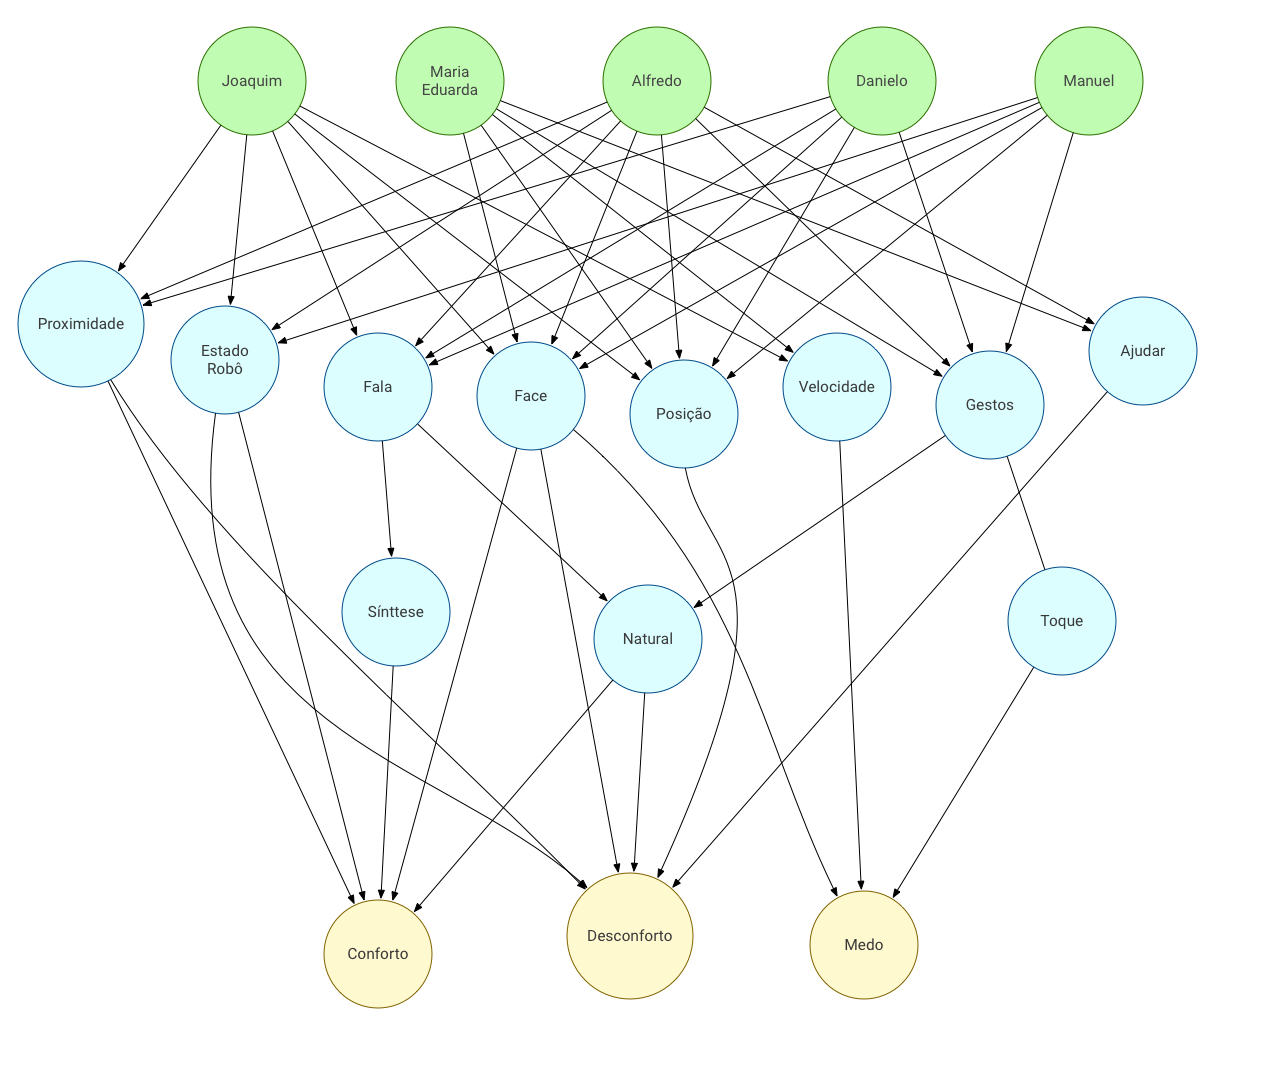
\includegraphics[width=\textwidth]{rb-thesis.png}
		\smallcaption{Fonte: Autor.}
		\label{fig:rb}
	\end{minipage}
\end{figure}

A partir de agora é preciso formalizar a rede bayesiana através de probabilidades, para que seja possível compreender cada um dos cálculos de inferência e diagnóstico realizados pelo mecanismo de autoavaliação do robô ao interagir com o usuário. As equações~\ref{eq:1}, \ref{eq:2}, \ref{eq:3}, \ref{eq:4}, \ref{eq:5}, \ref{eq:6}, \ref{eq:7}, \ref{eq:8}, \ref{eq:9} e \ref{eq:10} representam as probabilidades da rede bayesiana para cada uma das variáveis aleatórias mapeadas.

\begin{equation}
	\label{eq:1}
	P(P1), P(P2), \dots, P(PN)
\end{equation}

\begin{equation}
	\label{eq:2}
	P(H01|P1, P2, \dots, PN), P(H02|P1, P2, \dots, PN), \dots, P(HN|P1, P2, \dots, PN)
\end{equation}

\begin{equation}
	\label{eq:3}
	P(POS|H01, H02, \dots, HN)
\end{equation}

\begin{equation}
	\label{eq:4}
	P(VEL|H01, H02, \dots, HN)
\end{equation}

\begin{equation}
	\label{eq:5}
	P(ROT|H01, H02, \dots, HN)
\end{equation}

\begin{equation}
	\label{eq:6}
	P(FALA|H01, H02, \dots, HN)
\end{equation}

\begin{equation}
	\label{eq:7}
	P(GES|H01, H02, \dots, HN)
\end{equation}

\begin{equation}
	\label{eq:8}
	P(FACE|H01, H02, \dots, HN)
\end{equation}

\begin{equation}
	\label{eq:9}
	P(CONFORTO|POS, VEL, ROT, FALA, GES, FACE)
\end{equation}

\begin{equation}
	\label{eq:10}
	P(DESCONFORTO|POS, VEL, ROT, FALA, GES, FACE)
\end{equation}

É importante ressaltar que o efeito a ser medido é a experiência do usuário, pois é o principal interessado na interação com o robô. A grande preocupação em manter o foco no ser humano é por que existem poucos trabalhos que consideram exatamente a experiência do usuário na interação, conforme \citeonline{alenljung:2017} afirma em seu trabalho. A tomada de decisão para melhorar a experiência do usuário a partir a autoavaliação do robô não faz parte do escopo desta tese, porém uma lista com possíveis expansões em características a serem consideradas é apresentada na seção~\ref{sec:extracaocaracteristicas}. As variáveis para auxiliar melhor a identificação de características da interação podem complementar a quarta camada da rede bayesiana e por consequência aprimorar mais a automação da avaliação da experiência do usuário.

\section{Características para Expandir o \emph{Framework}}
\label{sec:extracaocaracteristicas}

Como apresentado no capítulo \ref{cap:proxemics}, existem diversas variáveis que podem auxiliar na extração de um perfil comportamental do indivíduo. \emph{Proxemics} tornam possível a extração de fatores comportamentais baseados na distância social entre o indivíduo e o robô. Esses fatores podem variar não só entre a posição física dos dois agentes, mas também na posição do corpo dos indivíduos, como por exemplo, a orientação dos ombros e troco em relação a posição do robô (linguagem corporal). Outro fator significante é a fixação entre olhares, este pode auxiliar no processo que determina o início e o fim de uma interação. O olhar também auxilia a determinar quem são os principais indivíduos na interação. Pode-se empregar o reconhecimento de expressões faciais para auxílio na análise do quanto a situação é confortável para o indivíduo, ou o quanto o usuário aprecia a interação. Existir uma avaliação em tempo real das reações deste indivíduo durante todo o processo de interação, auxilia na compreensão da experiência do usuário. Outra técnica para análise de conforto na interação é a avaliação da emoção através da voz da pessoa, ou através do uso de equipamento de eletroencefalografia~(EEG), porém este último é um método mais invasivo já que exige a adição de um equipamento na pessoa que interage com o robô.

É possível empregar diversos sensores que auxiliam a leitura e quantificação dessas variáveis. Sensores de captura de marcações de movimento, como Microsoft\textregistered\ Kinect\textregistered\ ou o ASUS\textregistered\ Xtion\textregistered, são utilizados para quantificar os valores comportamentais obtidos através das variáveis, que envolvem distância entre agentes e orientação de membros do indivíduo. Para realizar o reconhecimento de expressões faciais utiliza-se uma câmera de video, podendo assim executar uma leitura da face da pessoa em tempo de execução. As variáveis referentes a questão da fixação dos olhares dos agentes para identificar o início e o fim da interação, podem ser obtidas através de ambos sensores, sendo possível determinar a orientação da cabeça e torso do indivíduo, além de também a direção do olhar da pessoa para o robô. A voz do indivíduo para análise da emoção na interação é obtida através de um microfone direcional ou um arranjo de microfones, que amplifica a capacidade de percepção do robô em relação ao ambiente e a pessoa que interage com ele.

As variáveis aplicadas ao comportamento tem dependência do cenário de interação, porém as informações das variáveis etnográficas como idade, experiência computacional, sexo, local de origem, etnia, entre outras, são independentes do cenário. Existem alguns algoritmos na área de visão computacional que são capazes de identificar algumas variáveis etnográficas de maneira automática \cite{yang:2007, shan:2012, ylioinas:2012, samadi:2013, amaral:2014}, isso pode auxiliar no processo de expansão da rede bayesiana de maneira automática. Porém nem todas as informações podem ser obtidas de maneira automática ainda, então métodos como questionários ainda são necessários para melhor compreendimento do comportamento do usuário e qual sua experiência durante a interação.

Na seção~\ref{sec:variaveisindivíduo} são detalhados os conjuntos de variáveis etnográficas e comportamentais com uma breve explicação dos objetivos esperados de cada uma das variáveis em uma futura expansão do \emph{framework} de autoavaliação da experiência do usuário pelo robô. A seção~\ref{sec:variaveisrobo} detalha as variáveis consideradas para o perfil do robô, apresentando também uma explicação sobre os objetivos de cada uma. Essas seções são consideradas como um mapa de variáveis importante para estudos comportamentais em interação humano-robô social, podendo ser implementadas em futuros trabalhos.

\subsection{Selecionando Variáveis do Usuário}
\label{sec:variaveisindivíduo}

Essa seção apresenta os conjuntos de variáveis que são consideradas como a base de informações para desenvolvimento de estudos em interação humano-robô social. Dois conjuntos são apresentados, o conjunto de variáveis etnográficas, seguido pelo conjunto de variáveis comportamentais que é o principal foco deste trabalho.

\subsubsection{Conjunto de Variáveis Etnográficas}
\label{sec:variaveisetnograficas}

O objetivo das variáveis etnográficas é identificar qual a experiência social e computacional de cada indivíduo. Além da experiência, também pode-se obter informações sobre a idade, gênero, local de nascimento ou origem do indivíduo. Todas essas informações são relevantes para verificar a existência de uma possível relação entre as variáveis etnográficas e comportamentais, além da relevância cultural para estabalecer uma interação social de curta e longa duração. A lista apresentada a seguir define as variáveis etnográficas e uma breve explicação sobre o significado de cada uma das variáveis.

\begin{enumerate}
	\item \textbf{Idade}: informa a idade do indivíduo.
	\item \textbf{Gênero}: informa o sexo biológico do indivíduo.
	\item \textbf{Local de Nascimento}: informa qual o local de nascimento do indivíduo. Essa variável auxiliará a determinar a base cultural do indivíduo.
	\item \textbf{Etnia}: informa a origem da família do indivíduo. Outra variável que auxilia na determinação da base cultural do indivíduo.
	\item \textbf{Quantidade de \emph{Gadgets}}: informa a quantidade de \emph{gadgets} que o indivíduo possui, ajudando a identificar qual a experiência e o contato dele com a tecnologia.
	\item \textbf{Contato prévio com Robôs}: informa apenas se o indivíduo já possuiu algum contato com robôs. Auxiliará a determinar o contato com a tecnologia, principalmente com robôs que poderá influenciar no seu comportamento durante a interação.
	\item \textbf{Tipos de Robôs}: informa quais são os tipos de robôs que o indivíduo teve contato. Os tipos poderão ser robôs \emph{Pet}, Humanoides, Androides, Móveis, entre outros. Essa variável é um complemento da variável ``Contato prévio com Robôs''.
	\item \textbf{Quantidade de cidades visitadas}: informa a quantidade de cidades que o indivíduo já visitou além da sua cidade natal. É importante para identificar o contato com outros tipos de cultura. Isso poderá influenciar no comportamento definido por sua cultura.
	\item \textbf{Quantidade de cidades que morou}: informa a quantidade de cidades que o indivíduo já morou além da sua cidade natal. É importante para identificar a vivência com outros tipos de cultura. Isso poderá influenciar no comportamento definido por sua cultura.
	\item \textbf{Quantidade de países visitadas}: informa a quantidade de países que o indivíduo já visitou além da sua cidade natal. É importante para identificar o contato com outros tipos de cultura. Isso poderá influenciar no comportamento definido por sua cultura.
	\item \textbf{Quantidade de países que morou}: informa a quantidade de países que o indivíduo já morou além da sua cidade natal. É importante para identificar a vivência com outros tipos de cultura. Isso poderá influenciar no comportamento definido por sua cultura.
\end{enumerate}

Em diversos trabalhos da seção \ref{sec:proxemicsihr}, onde a questão cultural do indivíduo é abordada, são discutidos que influência a cultura provê sobre o comportamenteo do o indivíduo. A cultura é tratada como a origem do indivíduo~\cite{eresha:2013}. Entretanto, esta tese acredita que a questão cultural na vida de uma pessoa é mais abrangente. Ela está relacionada a experiência adquirida ao longo de sua vivência social, como por exemplo, países e cidades que o indivíduo visitou e viveu, o meio ao qual ele está inserido, sua profissão, entre outras informações. Dessa forma, o conjunto de variáveis apresentado na lista acima auxilia a mapear de forma abstrata a experiência social do indivíduo, com o intuito de verificar se o comportamento é menos dependente da origem do indivíduo e mais dependente de sua experiência tanto de vida, quanto de interação com o robô.

Algumas informações apresentadas nessa seção são adquiridas através do questionário pré-teste (vide seção~\ref{sec:questionarios}). Em trabalhos futuros poderão ser aplicados estudos para identificar essas informações de maneira interativa através do próprio robô.

\subsubsection{Conjunto de Variáveis Comportamentais}
\label{sec:variaveiscomportamentais}

Variáveis comportamentais tem como principal objetivo identificar o comportamento do indivíduo dentro do cenário exigido por uma determinada tarefa. Nessa tese o comportamento está diretamente relacionado com cenários de interação social. As variáveis comportamentais são coletadas a partir de informações sobre expressões corporais e faciais da pessoa, tornando possível uma análise com base em teorias de linguagem corporal e de microexpressões. Algumas possibilidades para analisar expressões corporais são discutidas no trabalho apresentado por \citeonline{lambert:2008}. O conjunto de variáveis comportamentais apresentados nessa seção podem ser utilizados não apenas para extrair o perfil do indivíduo, mas também para avaliar a ação realizada pelo robô ao interagir com o usuário. A lista apresentada a seguir define as variáveis comportamentais obtidas através da literatura e uma breve explicação sobre o objetivo de cada uma das variáveis.

\begin{enumerate}
	\item \textbf{Expressões Faciais}: é possível identificar se a reação do indivíduo foi positiva ou negativa, a partir de uma ação do robô. Existem seis expressões bases que combinadas formam diversas outras~\cite{bihan:2014}. Contudo, nesse trabalho será considerado apenas as seis expressões bases classificadas em dois grupos: expressões faciais positivas e expressões faciais negativas. O intuito dessa variável é realizar a avaliação da ação do robô com base nas expressões faciais do indivíduo.
	\item \textbf{Tempo de Transição entre as Zonas Sociais}: identificar o tempo que o indivíduo ficou confortável com a presença do robô a medida que esse diminuiu a distância entre eles.
	\item \textbf{Frequência do Olhar em direção ao Robô}: identificar se o indivíduo mantém o olhar ao robô, sendo possível saber se a interação está continua ou não. Isso pode influenciar se o robô está interagindo de maneira confortável ao indivíduo ou se esse está incomodado com a presença do robô.
	\item \textbf{Tempo do Olhar}: é possível mensurar o interesse do indivíduo durante a interação através do tempo que ele permanece com o olhar fixo no robô. Quanto maior o tempo do olhar, maior o interesse na interação do indivíduo.
	\item \textbf{Orientação dos ombros}: Auxilia a mensurar o interesse do indivíduo durante a interação, analisando se os ombros possuem a mesma orientação que a cabeça e também uma orientação em direção ao indivíduo que interage com o robô. Além disso, é possível determinar através do alinhamento do quadril com o ombro do indivíduo o ângulo de inclinação de seu torso. A inclinação do torso auxilia a identificar o interesse do indivíduo na interação, para isso basta verificar se ele está inclinado em direção ao robô para determinar um interesse positivo.
	\item \textbf{Orientação do quadril}: Auxilia a mensurar o interesse do indivíduo durante a interação. A orientação do quadril em direção ao robô ou na direção oposta auxilia a determinar o grau de interesse do indivíduo na interação. Quando mais alinhado à direção do robô, maior o interesse do indivíduo na interação.
	\item \textbf{Estilo da Voz}: é importante, pois pode determinar a reação que o indivíduo terá após a interação via áudio com o robô. Além disso, é possível determinar se o indivíduo está confortável ou não durante a interação, analisando o tom de sua voz ao responder o robô. Nesse trabalho, será considerado somente o canal de resposta ao indivíduo.
\end{enumerate}

As variáveis apresentadas acima podem auxiliar na descoberta do interesse em relação a interação. Algumas delas, como as que envolve o olhar, podem necessitar de equipamentos mais específicos para obter uma melhor acurácia na captura. Outras variáveis necessitam de técnicas e estudos direcionados para trazer a interação à um nível mais natural, como o caso da voz. Dessa forma, escolher quais variáveis trabalhar tem influência não só sobre o estudo realizado, como também nos equipamentos embarcados no robô. Tais equipamentos, podem influenciar em sua aparência e consequentemente na experiência que o usuário terá. Essas variáveis que influenciam sobre o robôs são apresentadas na seção~\ref{sec:variaveisrobo}, a seguir.

\subsection{Selecionando as Variáveis para o Robô}
\label{sec:variaveisrobo}
Além das variáveis referentes ao perfil do indivíduo, deve-se considerar também as informações sobre o robô uma vez que sua aparência pode influenciar na reação das pessoas durante a interação~\cite{hegel:2009}. Variáveis do robô podem auxiliar a identificar quais são os principais fatores que tornam a interação humano-robô uma boa experiência ao usuário e também uma experiência natural. Um conjunto de variáveis é apresentado com o objetivo de caracterizar fatores do robô, referente a sua aparência, que influenciam na interação social. Esse conjunto de variáveis é apresentado a seguir:

\begin{enumerate}
	\item \textbf{Altura}: A altura do robô para identificar a influência da diferença entre alturas de robôs e humanos.
	\item \textbf{Volume}: O volume ocupado pelo robô pode influenciar no conforto da interação, uma vez que quando o robô atingir uma zona social mais próxima do indivíduo pode causar uma sensação claustrofóbica a ele.
	\item \textbf{Tipo do Robô}: Segundo \citeonline{choi:2014}, robôs possuem dois tipos: Autônomos e Tele-operados. Essa variável define o quanto de intervenção humana é necessário para que o robô possa executar a tarefa objetivo.
	\item \textbf{Classificação do Robô}: Segundo \citeonline{dobra:2014} classificar um robô é uma tarefa muito complexa e pode envolver diversas variáveis. Dessa forma, para essa tese será considerado uma classificação mais simples. O robô deve ser classificado como: fixo, móvel com rodas, móvel bípede, móvel quadrupede, móvel com manipuladores. Outras classificações podem ser inseridas conforme a necessidade e inclusão de novos robôs.
	\item \textbf{Aparência Física}: Essa variável descreve se o robô possui uma aparência amigável ou agressiva.
	\item \textbf{Nível de Ruído}: Determina qual o nível de ruído que os atuadores do robô podem gerar de tal forma, que possa influenciar na interação humano-robô. Como exemplo, pode-se citar o Big Dog~\footnote{http://www.bostondynamics.com/robot\_bigdog.html}, da Darpa Robotics, que é movido através de um motor diesel e seus atuadores pneumáticos e hidráulicos apresentam um alto grau de ruído.
\end{enumerate}

Além das variáveis que definem as características, existe o mapeamento das ações que o robô irá executar para que informações sobre a reação da pessoa sejam investigadas e compreendidas a fim de fazer um modelo computacional para raciocínio do robô. As variáveis que compõem as informações do perfil comportamental do robô são:

\begin{enumerate}
	\item \textbf{Aproximação}: Forma de aproximação do robô ao indivíduo. Pode ser classificada entre rápida, devagar, brusca ou suave.
	\item \textbf{Movimentação do Manipulador}: Caso exista um manipulador deve descrever como é feita a movimentação do manipulador em direção ao usuário. A classificação pode ser feita entre brusca e suave; ou em relação a sua amplitude, como longo e curto.
	\item \textbf{Estilo de Voz}: Ao emitir algum tipo de som o robô deverá manter um estilo de voz para que seja possível simbolizar qual o tipo de mensagem ele deseja falar. A classificação será feita de maneira simplificada, considerando apenas se é um estilo educado ou agressivo.
	\item \textbf{Volume de Voz}: Ao emitir um som, o robô deve saber qual o volume adequada considerando a interação, ambiente e distância do segundo agente. Uma classificação simples pode ser utilizada, como por exemplo, alto e baixo.
	\item \textbf{Expressão Facial}: Ao iniciar o contato visual com o indivíduo, pode ocorrer diversas expressões do robô na tentativa de manter o conforto do indivíduo durante o processo de interação. Simplificando as expressões, de maneira similar ao apresentado na seção~\ref{sec:variaveiscomportamentais}, são consideradas apenas dois tipos de expressões realizadas pelo robô: amistoso e não-amistoso. As expressões faciais do robô serão executadas através do \emph{tablet} acoplado nele, conforme descrito na seção~\ref{sec:robo}.
\end{enumerate}

Caso seja necessário deve-se adicionar novas variáveis a esse conjunto e essa adição não afetará ao método apresentado como proposta dessa tese, auxilirá sim em uma melhor acurácia da avaliação sobre a experiência do usuário na interação social. Essas informações a partir de um momento em que forem automatizadas a sua detecção, poderão retro alimentar as tabelas de propabilidades condicionais da rede bayesiana melhorando cada vez mais o diagnóstico do conforto ou desconforto do usuário na interação com o robô.
